\documentclass{standalone}
\usepackage{pgfplots}
\pgfplotsset{width=9cm, compat=1.5}
\begin{document}
	\begin{tikzpicture}
	\begin{axis}[
	xlabel=$\varepsilon$,
	ylabel=Magnetizaci\'on $(\mu_B)$]
	
	\addplot table [x=e, y=magn] {magn.dat};
	\node at (450,140) {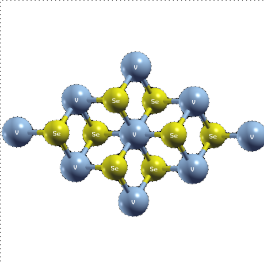
\includegraphics[scale=0.17]{est_0.0}};
	\node at (700,20) {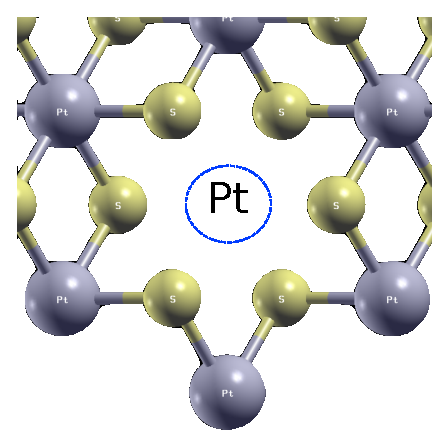
\includegraphics[scale=0.2]{est_0.05}};
	%\node at (150,30) {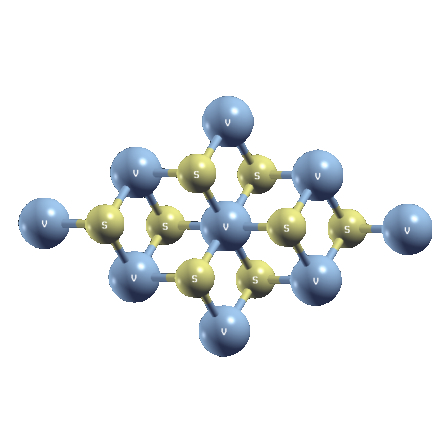
\includegraphics[scale=0.2]{est_-0.05}};
	%\draw[->, color=black, very thick](100,65)--(10,90);
	\draw[->, color=black, very thick](830,10)--(960,2);
	\draw[->, color=black, very thick](480,210)--(500,240);
	\end{axis}
	
	\end{tikzpicture}
\end{document}
